\documentclass[xcolor=dvipsnames]{beamer}
\usepackage[utf8]{inputenc}

\usepackage{amsfonts}
\usepackage{amsmath}
\usepackage{amssymb}
\usepackage{amsthm}
\usepackage{minted}
\usepackage{tikz}
\usepackage{graphicx}
\usepackage{optidef}

\usetheme{Rochester}

\definecolor{CSHpink}{rgb}{0.69020, 0.09804, 0.49412}
\definecolor{CSHblue}{rgb}{0.25098, 0.29412, 0.41176} 
\definecolor{CSHgrey}{rgb}{0.95686, 0.95686, 0.96471}

\setbeamercolor{palette primary}{bg=CSHpink,fg=white}
\setbeamercolor{palette secondary}{bg=CSHpink,fg=white}
\setbeamercolor{palette tertiary}{bg=CSHpink,fg=white}
\setbeamercolor{palette quaternary}{bg=CSHpink,fg=white}
\setbeamercolor{structure}{fg=CSHpink} 
\setbeamercolor{section in toc}{fg=CSHpink} 
\setbeamercolor{background canvas}{bg=CSHblue}
\setbeamercolor{normal text}{fg=CSHgrey}
\setbeamercolor{example text}{fg=CSHpink}
\setbeamercolor{alerted text}{fg=CSHgrey}
\setbeamercolor{theorem text}{fg=CSHblue}
\setbeamercolor{subsection in head/foot}{bg=CSHblue,fg=white}
\setbeamercolor{block title}{fg=CSHgrey, bg=CSHpink}
\setbeamercolor{block body}{fg=CSHblue}

\title{An Introduction to Information Theory with Applications to Machine Learning}
\date{\today}
\author[Cade]{Cade Reinberger}
\institute[CSH]{RIT Computer Science House}

\begin{document}
	
	\begin{frame}
		\titlepage
	\end{frame}
	
	\begin{frame}{Outline}
		\tableofcontents
	\end{frame}
	
	\section{Motivating Information Entropy}
	
	\subsection{$\alpha$-weighted coins}
	\begin{frame}
	    \frametitle{$\alpha$-weighted coins}
		We begin with a motivating example
		\begin{itemize}
			\item Let $\alpha \in \mathbb{R}$ be a real paramater with $0 \leq \alpha \leq 1$
			\pause
			\item We define an $\alpha$-weighted coin, or simply an $\alpha$-coin, to be a coin which lands heads ($H$) with probability $\alpha$ and tails ($T$) with probability $1 - \alpha$
			\pause
			\item We want to encode the result of this coin toss as information
		\end{itemize}
	\end{frame}
	
	\subsection{Binary Trees}
	\begin{frame}
	    \frametitle{Binary Trees}
		\begin{itemize}
			\item Our goal is to encode the outcome of this coin toss as a sequence of 0s and 1s with optimal efficiency
			\pause
			\item We use a binary tree to do this encoding. 
			\pause
			\item a \textit{binary tree} is a recursive graph-like data structure with parent nodes and leaves. Each parent node contains two children, starting with one node known as the \textit{root}, and each leaf contains no children but a value
		\end{itemize}
	\end{frame}
	
	\begin{frame}[fragile]
	\frametitle{Binary Trees}
    	\begin{center}
            \begin{minted} 
            [
            frame=lines,
            framesep=2mm,
            baselinestretch=1.2,
            bgcolor=LightGray,
            fontsize=\footnotesize,
            linenos
            ]
            {python}
            
class binary_tree_node:
    def __init__(self, is_leaf, left, right, val):
        if is_leaf:
            self.is_leaf = True
            self.left_child = None
            self.right_child = None
            self.val = val
        else:
            self.is_leaf = False
            self.left_child = left
            self.right_child = right
            self.val = None
            
    	    \end{minted}
		\end{center}
	\end{frame}
	
	\begin{frame}
	\frametitle{Binary Trees}
    	\begin{center}
    	    \begin{tikzpicture}[very thick,level/.style={sibling distance=60mm/#1}]
                \begin{scope}[scale=.9, xshift=-5cm]
                    \node [vertex] (r){$\bullet$}
                      child {
                        node [vertex] (a) {$\bullet$}
                        child {
                          node [vertex] {$\bullet$}
                          child {
                            node [vertex] {$\bullet$}
                            child {node [vertex] {$\bullet$}
                                child{node[vertex]{$\text{E}$}}
                                child{node[vertex]{$\text{F}$}}}
                            child[missing]{}
                            child {node [vertex] {$\bullet$}
                                child{node[vertex]{$\text{G}$}}
                                child{node[vertex]{$\text{H}$}}}
                          }
                          child {node [vertex] {$\text{B}$}}
                        }
                        child {
                          node [vertex] {$\bullet$}
                          child {node [vertex] {$\text{C}$}}
                          child {node [vertex] {$\text{D}$}}
                        }
                      }
                      child {
                        node [vertex] {$\text{A}$}
                        };
                \end{scope}
            \end{tikzpicture}
    	\end{center}
	\end{frame}
	
	\begin{frame}
	\frametitle{Binary Trees}
	    \begin{itemize}
	        \item Binary Trees are not only natural to express this encoding, but are more or less a fully accurate representation of the problem (that is, encodings are equivalent to Binary Trees). 
	        \pause
	        \item ``Normal" binary trees in most of CS (such as BSTs), can contain a value at \textit{all} nodes, not just leaves. Why isn't that true for encoding binary information?
	        \pause
	        \item Because to read that as an encoding, the encoder has to recognize at the end of the encoding string that it has ended. Thus, implicitly, saying some string has ended adds an extra termination bit of information at the end. 
	    \end{itemize}
	\end{frame}
	
	
	\subsection{Encoding Coin Flips}
	\begin{frame}
	\frametitle{Encoding Coin Flips}
	    \begin{itemize}
	        \item For our goal of encoding the result of an $\alpha$-coin flip using binary trees, the answer is very boring. 
	        \pause
	        \item For $\alpha \neq 0, 1$, there's one obvious best encoding
	        \begin{center}
    	        \begin{tikzpicture}
                    \node [vertex] (r){$\bullet$}
                  child {node [vertex]  {\text{T}}}
                  child{node[vertex]{\text{H}}};
                \end{tikzpicture}
	        \end{center}
	        \pause
	        \item Good night everybody
	    \end{itemize}
	\end{frame}
	
	\begin{frame}
	\frametitle{Encoding Coin Flips}
	    \begin{itemize}
	        \item For our goal of encoding the result of an $\alpha$-coin flip using binary trees, the answer is very boring. 
	        \item For $\alpha \neq 0, 1$, there's one obvious best encoding
	        \begin{center}
    	        \begin{tikzpicture}
                    \node [vertex] (r){$\bullet$}
                  child {node [vertex]  {\text{T}}}
                  child{node[vertex]{\text{H}}};
                \end{tikzpicture}
	        \end{center}
	        \item What went wrong?
	    \end{itemize}
	\end{frame}
	
	\begin{frame}
	\frametitle{Encoding Coin Flips}
    	\begin{itemize}
    	    \item Well, imagine that $\alpha = 1 - \varepsilon$ with $\varepsilon$ small
    	    \pause
    	    \item Maybe if you toss the coin once, $T$ is not avoidable since $\varepsilon$ is not neglible, but say you toss the coin 10 times. 
    	    \item $\varepsilon^{10}$ will be pretty well negligible, so there ought to be at least effectively one less outcome ($TTTTTTTTTT$) than in the case of $\alpha = \frac{1}{2}$, when all strings are equally likely.
    	    \pause
    	    \item Thus, we might expect that we can somehow do better encoding 10 coin tosses than 1 coin toss. 
    	\end{itemize}
	\end{frame}
	
	\begin{frame}
	\frametitle{Encoding Coin Flips}
	\begin{itemize}
	    \item Let's imagine encoding the result of 3 $.9$-coin flips in a binary tree, such that we minimize the expected length of the message. 
	    \begin{center}
       	    \begin{tikzpicture}[scale=.6,very thick,level/.style={sibling distance=100mm/#1}]
                \begin{scope}[scale=.9, xshift=-5cm]
                    \node [vertex] (r){$\bullet$}
                      child {
                        node [vertex] (a) {$\bullet$}
                        child {
                          node [vertex] {$\bullet$}
                          child {
                            node [vertex] {$\bullet$}
                            child {node [vertex] {$\bullet$}
                                child{node[vertex]{$\text{HTT}$}}
                                child{node[vertex]{$\text{THT}$}}}
                            child[missing]{}
                            child {node [vertex] {$\bullet$}
                                child{node[vertex]{$\text{TTH}$}}
                                child{node[vertex]{$\text{TTT}$}}}
                          }
                          child {node [vertex] {$\text{HHT}$}}
                        }
                        child {
                          node [vertex] {$\bullet$}
                          child {node [vertex] {$\text{HTH}$}}
                          child {node [vertex] {$\text{THH}$}}
                        }
                      }
                      child {
                        node [vertex] {$\text{HHH}$}
                        };
                    \end{scope}
            \end{tikzpicture}
	    \end{center}
	\end{itemize}
	\end{frame}
	
	\begin{frame}
	\frametitle{Encoding Coin Flips}
    	\begin{itemize}
        	\begin{center}
        	    \begin{tabular}{|c|c|c|c|c|}
        	         \hline
        	         Result & Encoding & Length & Probability & $\%$  \\
        	         \hline
        	         \hline
        	         HHH & 1 & 1 & (.9)(.9)(.9) & $72.9\%$ \\ 
        	         \hline
        	         HHT & 001 & 3 & (.9)(.9)(.1) & $8.1\%$ \\ 
        	         \hline
        	         HTH & 010 & 3 & (.9)(.1)(.9) & $8.1\%$ \\ 
        	         \hline
        	         THH & 011 & 3 & (.1)(.9)(.9) & $8.1\%$ \\ 
        	         \hline
        	         HTT & 00000 & 5 & (.9)(.1)(.1) & $0.9\%$ \\ 
        	         \hline
        	         THT & 00001 & 5 & (.1)(.9)(.1) & $0.9\%$ \\ 
        	         \hline
        	         TTH & 00010 & 5 & (.1)(.1)(.9) & $0.9\%$ \\ 
        	         \hline
        	         TTT & 00011 & 5 & (.1)(.1)(.1) & $0.1\%$ \\
        	         \hline
        	    \end{tabular}
        	\end{center}
        	\pause
        	\vphantom{CSH}
    	    \item So our expected length is (.729)(1) + (3)(.081)(3) + (3)(.009)(5) + (.001)(5) = \textbf{1.598}
    	\end{itemize}
	\end{frame}
	
	\begin{frame}
	\frametitle{Encoding Coin Flips}
	    \begin{itemize}
	        \item So we can encode 3 idependent trials of a $.9$-coin with less than 3 bits, on average. 
	        \pause
	        $$\frac{1.598}{3} = .532667$$
	        \pause
	        \item Thus, there's not really a full bit of information in tossing a coin with $\alpha = .9$
	    \end{itemize}
	\end{frame}
	
	
	\subsection{Information Entropy}
	
	
	\begin{frame}
	\frametitle{Information Entropy}
    	\begin{itemize}
    		\item As I encode $n$ independent instances of an $\alpha$-coin, the minimum average length is a non-increasing function of $n$, so what happens to it in the long term
        	\pause
        	\item Somewhat miraculously, we have that  the best average length approaches an actual limit. 
    	\end{itemize}
	\end{frame}
	
	\begin{frame}
	\frametitle{Information Entropy}
    	\begin{theorem}[Shannon's Source Coding Theorem, Bernoulli Trial]
	    Let $\mathbb{T}_n$ denote the set of all binary trees with $2^n$ leaves, let $C_n \in \{H, T\}^n$ be a random variable, the result of $n$ iid $\alpha$-coin tosses, and let $\operatorname{len}_\tau(C_n)$ for a binary tree $\tau \in \mathbb{T}_n$ denote the length of encoding $C_n$ within the binary tree $\tau$. Then $$ \lim_{n \to \infty}  \min_{\tau \in \mathbb{T}_n} \frac{\mathbb{E}[\operatorname{len}_{\tau}(C_n)]}{n} = H$$ for some real constant $H \geq 0$        	
	    \end{theorem}
	\end{frame}
	
	\begin{frame}
	\frametitle{Information Entropy}
    	\textit{Proof.} The minimum expected length is monotone decreasing and bounded below by 0, the result follows trivially from the monotone convergence theorem
	\end{frame}
	
	\begin{frame}
	\frametitle{Information Entropy}
	\begin{itemize}
	    \item This limit $H$ is called the \textit{information entropy} of the coin toss, in units of bits (or Shannons). 
	\end{itemize}
	\end{frame}
	
	
	\subsection{Computing Information Entropy}
	
	
	\begin{frame}
	\frametitle{Computing Information Entropy}
	    \begin{itemize}
	        \item So why is Shannon famous?
	        \pause
	        \item We can compute the value of $H$.
	        \pause
	        \item Shannon's original computation was rather difficult, and was specifically considering information in Markov Chains. In fact, if you're careful about the logarithm as having negative concavity and so-forth, you can simply prove that you can get arbitrarily close to $H$ and never do better than $H$.
	        \pause
	        \item We're going to consider a slightly less rigorous derivation. 
	    \end{itemize}
	\end{frame}
	
	\begin{frame}
	\frametitle{Computing Information Entropy}
	\begin{itemize}
	    \item Consider some binary tree $\tau \in \mathbb{T}_n$ encoding $C_n$. 
	    \pause
	    \item We claim first that we can determine the expected length of this encoding by simply considering the average lengths of $H$ and $T$, and weighting appropriately. 
	    \pause
	    \item We could take this as something of a definition of ``average" in a suitable sense, but it's not so tough to see that this is just the arithmetic mean of the length of all instances of $H$ in the encoding in a technical sense.  
	    \pause
	\end{itemize}
	\end{frame}
	
	\begin{frame}
	\frametitle{Computing Information Entropy}
	    \begin{itemize}
	    \item So, in the asymptotic, we can ditch the trees themselves and think in terms of \textit{average lengths.}
	    \pause
	    \item Besides the fact this length isn't technically defined, we also haven't shown that we can generate binary trees that create average lengths (pointwise) convergent, to some set of averages. 
	    \pause
	    \item Surely not \textit{any} set of lengths will do. Which ones will?
		\end{itemize}
	\end{frame}
	
    \begin{frame}
	\frametitle{Computing Information Entropy}
    	\begin{center}
    	    \begin{tikzpicture}[very thick,level/.style={sibling distance=60mm/#1}]
                \begin{scope}[scale=.9, xshift=-5cm]
                    \node [vertex] (r){$\bullet$}
                      child {
                        node [vertex] (a) {$\bullet$}
                        child {
                          node [vertex] {$\bullet$}
                          child {
                            node [vertex] {$\bullet$}
                            child {node [vertex] {$\bullet$}
                                child{node[vertex]{$\text{E}$}}
                                child{node[vertex]{$\text{F}$}}}
                            child[missing]{}
                            child {node [vertex] {$\bullet$}
                                child{node[vertex]{$\text{G}$}}
                                child{node[vertex]{$\text{H}$}}}
                          }
                          child {node [vertex] {$\text{B}$}}
                        }
                        child {
                          node [vertex] {$\bullet$}
                          child {node [vertex] {$\text{C}$}}
                          child {node [vertex] {$\text{D}$}}
                        }
                      }
                      child {
                        node [vertex] {$\text{A}$}
                        };
                \end{scope}
            \end{tikzpicture}
    	\end{center}
	\end{frame}
	
	\begin{frame}
	\frametitle{Computing Information Entropy}
	    \begin{itemize}
	        \item We want to define some invariant, to understand the lengths of this tree. 
	        \pause
	        \item An easy invariant would be a sum of some function of depth. 
	        \pause
	        \item Such a sum would necessarily be invariant under bifurcation of a node, and thus if it's just a function of depth must half. 
	        \pause
	        \item There an infinite number of such invariant you could define based on the constant of proportionality, but the simplest is to sum simply $2^{-\text{(depth)}}$
	        \pause And considering the simplest binary tree, one with just a single node of depth zero, this sum may be one. 
	    \end{itemize}
	\end{frame}
	
	\begin{frame}
	\frametitle{Computing Information Entropy}
    	\begin{theorem}[Kraft-McMillan Inequality, Full Binary Trees]
	    Some tuple of number $(\ell_1, \ell_2, \dots, \ell_n)$ can form the depth of nodes on some valid binary tree $\tau$ if and only if $$ \sum_{k=1}^n 2^{-\ell_k} = 1$$      	
	    \end{theorem}
	\end{frame}
	
	\begin{frame}
	\frametitle{Computing Information Entropy}
    \textit{Proof (Necessity).} We use strong induction on the maximum depth. The sum is invariant under bifurcation, so if we ``combine" a pair of leaves into a lead of depth 1 lower, that leaves the sum unchanged. Do that for all nodes of maximum depth, and the depth is reduced. The base case is the trivial tree which clearly holds. 
    
    \textit{Proof (Sufficiency).} Simply consider the binary tree that always has children up to some fixed maximum depth, larger than the maximum of $\{\ell_k | k \in \mathbb{Z} \cap [1, n] \}$. Then simply keep going left up to depth $\ell_1$, then go left as much as you can, only stopping if you already reach a terminal leaf to go right. This process will yield such a tree. (Exercise: prove it rigorously). 
	\end{frame}
	
	\begin{frame}
	\frametitle{Computing Information Entropy}
	    \begin{itemize}
	        \item This gives us a regime for computing information entropy for an $\alpha$-coin!
	        \pause
	        \item Consider average depths $\ell_H$ and $\ell_T$ that are suitable for binary trees (in the sense of satisfying Kraft's inequality). 
	        \pause
	        \item Find the minimum average length among all such $\ell_H$ and $\ell_T$
	    \end{itemize}
	\end{frame}
	
	\begin{frame}
	\frametitle{Computing Information Entropy}
    	\begin{itemize}
    	    \item Thus we have $$ H = \min_{(\ell_H, \ell_T) \ \in \ \{(\ell_H, \ell_T) \left| \ 2^{-\ell_H} + 2^{-\ell_T} = 1  \}\right.}\left(\alpha \ell_H + (1-\alpha ) \ell_T\right) $$
    	    \pause
    	    \item Solving Kraft's inequality for $\ell_T$ gives us simply that $$ \ell_T = -\log_2\left( 1 - 2^{-\ell_H} \right)$$
    	    \pause
    	    \item Thus our problem is reduced to the 1-dimensional minimization problem $$ \min_{\ell_H} \left( \alpha \ell_H - (1 - \alpha) \log_2\left( 1 - 2^{-\ell_H} \right) \right)$$
    	\end{itemize}
	\end{frame}
	
	\begin{frame}
	\frametitle{Computing Information Entropy}
    	\begin{itemize}
    	    \item We can do this with some elementary calculus \begin{align*}
    	         & \frac{\text{d}}{\text{d}\ell_H} \left( \alpha \ell_H - (1 - \alpha) \log_2\left( 1 - 2^{-\ell_H} \right) \right) \\ = \ & \alpha - (1 - \alpha) \frac{\text{d}}{\text{d}\ell_H} \log_2\left( 1- 2^{-\ell_H} \right) \\ = \ & \alpha - \frac{1 - \alpha}{2^{\ell_H} - 1}
    	    \end{align*}
    	    \pause
    	    \item Setting this equal to 0 we get\begin{align*}
    	        \ell_H &= -\log_2(\alpha) \\  \ell_T  &= -\log_2(1-\alpha)\end{align*} 
    	\end{itemize}
	\end{frame}
	
	\begin{frame}
	\frametitle{Computing Information Entropy}
	\begin{itemize}
	    \item Thus, the information entropy of an $\alpha$ coin is $$ \boxed{H = -\alpha \log_2(\alpha) - (1-\alpha) \log_2(1-\alpha)} $$
	    \pause
	\end{itemize}
    	\begin{center}
    	    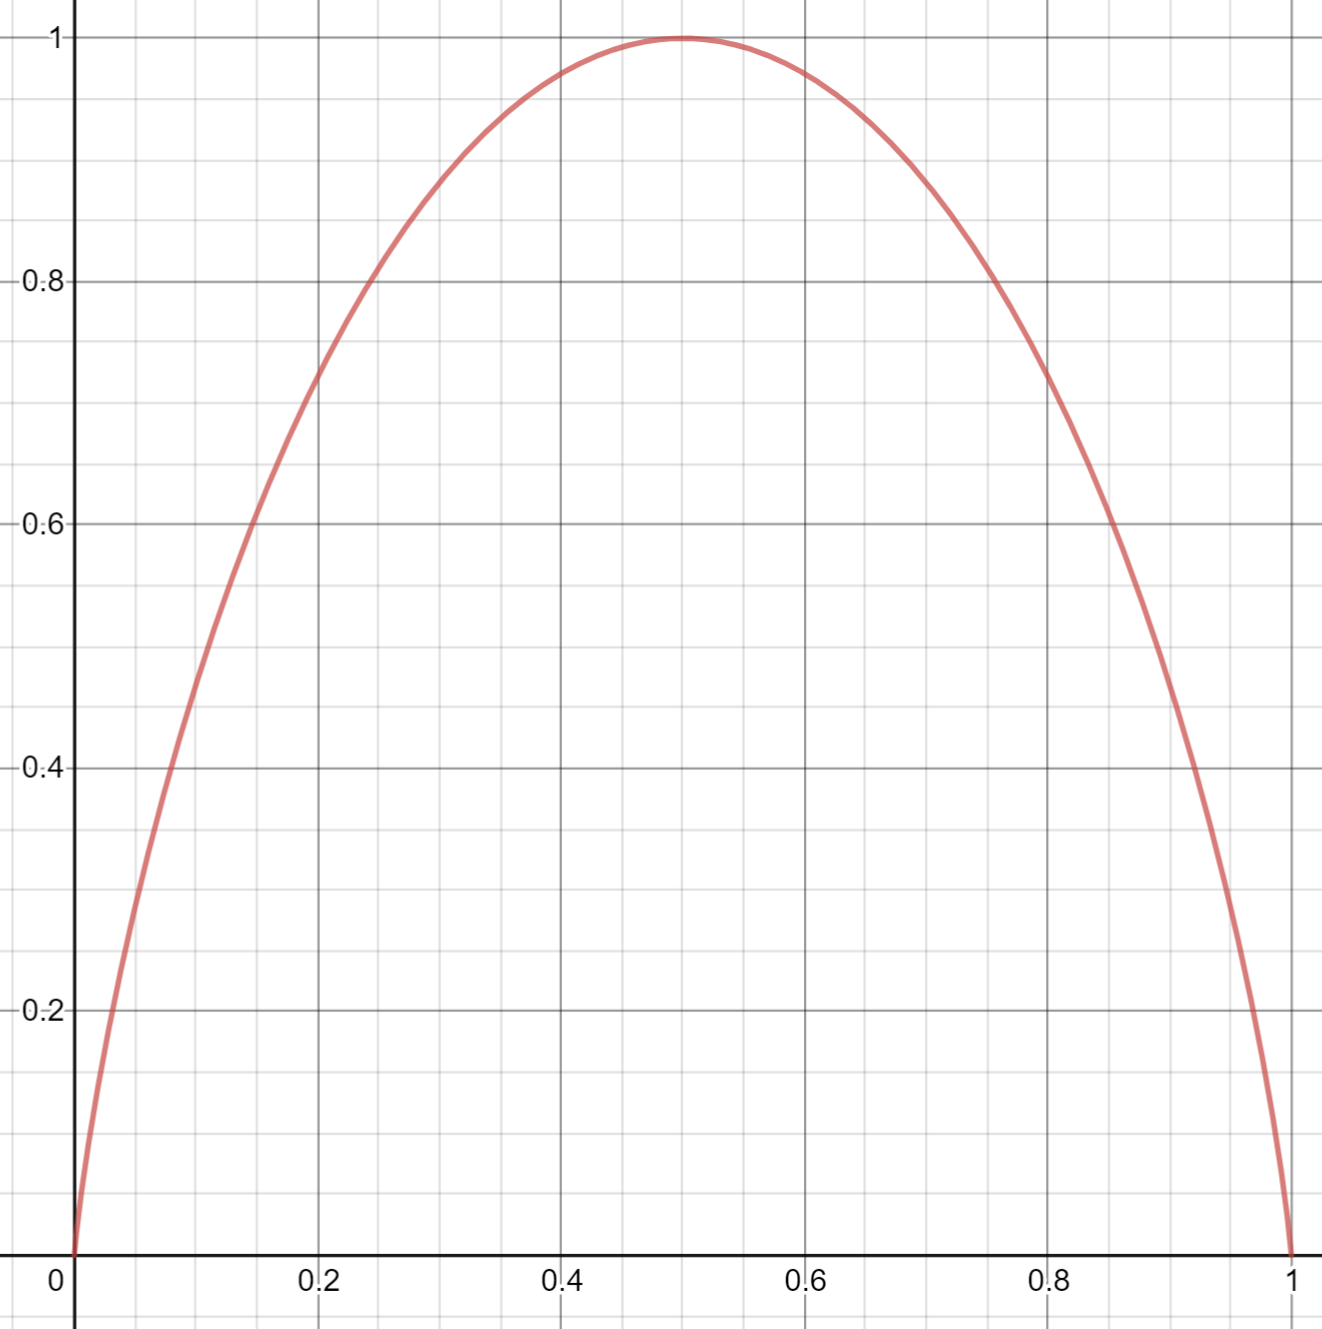
\includegraphics[scale=.3]{ent.PNG}
    	\end{center}
	\end{frame}
	
	\begin{frame}
	\frametitle{Computing Information Entropy}
    	\begin{itemize}
    	    \item Great. So we've done a bunch of calculation, and solved only this one very particular problem of entropy. :(
    	    \pause 
    	    \item But in fact, it is easy to adapt this method to any random variable with a finite image (set of possible values it could take). 
    	    \pause
    	    \item Simply assign all values the RV could take with an average length , so that all the lengths satisfy Kraft's inequality, and then find the minimum expected length over all such values. 
    	\end{itemize}
	\end{frame}
	
	\begin{frame}
	\frametitle{Computing Information Entropy}
	\begin{itemize}
	    \item Let $X$ be a random variable taking values $x_1, x_2, \dots, x_n$ with probabilities $p_1, p_2, \dots, p_n$. 
	    \pause
	    \item Then it's entropy is given by the constrained optimization problem in $n$ real dimensions 
            \begin{mini*}|s|
                {\ell_1, \ell_2, \dots, \ell_n}{\sum_{k=1}^np_k \ell_k}
                {}{}
                \addConstraint{\sum_{k=1}^n 2^{-\ell_k} = 1}
            \end{mini*}
        where $\ell_k$ denotes the average length assigned to $x_k$. 
        \pause
        \item We can solve this problem using the method of lagrange multipliers. 
    	\end{itemize}
	\end{frame}

	\begin{frame}
	\frametitle{Computing Information Entropy}
	    \begin{itemize}
	        \item We define the Lagrangian function $$\mathcal{L}(\ell_1, \ell_2, \dots, \ell_n, \lambda)  = \sum_{k=1}^n p_k \ell_k - \lambda \sum_{k=1}^m2^{-\ell_k} $$
	        \pause
	        \item Differentiating yields $$\frac{\partial \mathcal{L}}{\partial{\ell_k}} = p_k + \lambda\ln(2)2^{-\ell_k}$$
	        \pause
	        \item Setting that equal to zero gives $$ \ell_k = - \log_2 \left( \frac{-p_k}{\lambda \ln(2)} \right) $$
	    \end{itemize}
	\end{frame}
	
	\begin{frame}
	\frametitle{Computing Information Entropy}
    	\begin{itemize}
    	    \item Next we re-paramaterize our Lagrange multiplier, setting $$\hat{\lambda} = \frac{-1}{\lambda \ln(2)} $$
    	    \pause
    	    \item This yields $$ \ell_k = - \log_2\left( \hat{\lambda}p_k\right)$$
    	    \pause 
    	    \item Subbing this into our constraint gives $$ \sum_{k=1}^n 2^{-\ell_k} = \sum_{k=1}^n 2^{\log_2\left(\hat{\lambda p_k} \right)} = \hat{\lambda} \sum_{k=1}^n p_k = \hat{\lambda} = 1 $$
    	    \pause
    	    \item It follows that the optimizer is given simply by $$ \ell_k = -\log_2(p_k) $$
    	\end{itemize}
	\end{frame}
	
	\begin{frame}
	\frametitle{Computing Information Entropy}
	Thus, we have that the information entropy of a random variable taking values $x_1, x_2, \dots, x_n$ with probabilities $p_1, p_2, \dots, p_n$ is simply $$ \boxed{H = -\sum_{k=1}^n p_k \log_2(p_k)} $$
	\end{frame}
	
	
	\subsection{An Alternative Characterization}
	\begin{frame}
	\frametitle{An Alternative Characterization}
	    \begin{itemize}
	        \item So, this is a beautiful result. 
	        \pause
	        \item It is however, quite involved to make rigorous.
	        \pause
	        \item So, now that we have this pinned down a bit, it's nice to have an alternative characterization of information entropy that is 
	            \begin{enumerate}
	                \item Easier to prove formally
	                \item Coincident with our above result
	            \end{enumerate}
	    \end{itemize}
	\end{frame}
	
	\begin{frame}
	\frametitle{An Alternative Characterization}
	\begin{itemize}
    	\item  The idea is quite intuitive. For simplicity, we again begin with the simple case of the $\alpha$-coin. 
    	\pause
    	\item In particular, consider the result of $\ell$ iid $\alpha$-coin tosses. There are $2^n$ possible strings, but many of those are very unlikely. 
    	\pause
    	\item Let's consider $\ell$ large, and think about asymptotically how many of these strings are possible? 
	\end{itemize}
	\end{frame}
	
	\begin{frame}
	\frametitle{An Alternative Characterization}
	    \begin{itemize}
	        \item This distribution is incidentally well-understood. It's sum is a \textit{binomial} distribution. 
	        \pause
	        \item By the strong law of large numbers (say), we know that we need to consider strings that have roughly $\alpha \ell$ heads, those are the ones with non-negligible likelihood
	        \item We can compute the number of those, with binomial coefficients. 
	    \end{itemize}
	\end{frame}
	
	\begin{frame}
	\frametitle{An Alternative Characterization}
	    \begin{itemize}
	        \item We have a string of length $\ell$ with $0 \leq h \leq \ell$ heads. Equivalently, we  choose $h$ heads from the set of $\ell$ characters.
	        \pause 
	        \item We can generate such a set by undergoing a full permutation of all $\ell$ elements in the set (or think of their indices if you prefer), and taking the first $h$ as the chosen set. 
	        $$ \left. \vphantom{\int} \underbrace{\bullet \quad \bullet \quad \bullet \quad \bullet \quad \bullet \quad \bullet}_h \enspace \right| \enspace \underbrace{\bullet \quad \bullet \quad \bullet \quad \bullet \quad \bullet \quad \bullet \quad \bullet \quad \bullet \quad \bullet}_{\ell - h} $$
	        \pause 
	        \item The chosen set is invariant under permutations of the first $h$ and the last $\ell - h$, so we have to divide out by the number of those, but any other permutation that doesn't break down into two of those will break the set. \pause $$ \displaystyle {\ell \choose h} = \frac{\ell!}{h!(\ell - h)!} $$
	    \end{itemize}
	\end{frame}
	
	\begin{frame}
	\frametitle{An Alternative Characterization}
    	\begin{itemize}
    	    \item It follows pretty simply that our entropy ought to be asymptotically the number of bits needed to encompass all of the states with a number of heads equal to the mean as a ratio of $\ell$.  $$ H = \lim_{\ell \to \infty}\frac{\displaystyle \log_2 \left({\ell \choose \alpha \ell}\right)}{\ell} \pause = \lim_{\ell \to \infty} \frac{\displaystyle \log_2\left(\frac{\ell!}{(\alpha \ell)!(\ell - \alpha \ell)!}\right)}{\ell}$$
    	    \pause
    	    \item We can use \textit{Stirling's Approximation}, an asymptotic result about the factorial. $$ n! \sim \sqrt{2\pi n} \left(\frac{n}{e}\right)^n$$
    	\end{itemize}
	\end{frame}
	
		\begin{frame}
	    \frametitle{An Alternative Characterization}
            $$H = \lim_{\ell \to \infty}\frac{\displaystyle \log_2 \left({\ell \choose \alpha \ell}\right)}{\ell} \pause = \lim_{\ell \to \infty} \frac{\displaystyle \log_2\left(\frac{\ell!}{h!(\ell - h)!}\right)}{\ell} $$
            \pause
	        \resizebox{.95\hsize}{!}{$$ = \lim \limits_{\ell \to \infty} \frac{ \displaystyle \log_2\left( \frac{\displaystyle \sqrt{2\pi \ell} \ell^\ell e^{-\ell}}{\displaystyle \left(\sqrt{2\pi \alpha\ell}(\alpha\ell)^{\alpha\ell} e^{-\alpha \ell}\right)\left(\sqrt{2\pi (1-\alpha)\ell}((1-\alpha)\ell)^{(1-\alpha)\ell} e^{-(1-\alpha)\ell}\right)}\right)}{\displaystyle \ell} $$}
	        \pause 
	        $$ =\lim_{\ell \to \infty} \frac{\displaystyle \log_2\left( \frac{1}{\sqrt{2\pi\alpha(1-\alpha)\ell} \alpha^{\alpha\ell}(1-\alpha)^{(1-\alpha)\ell}} \right)}{\ell}$$ 
	        \pause 
	         $$ = \lim_{\ell \to \infty} \frac{\ell \left(-\alpha \log_2(\alpha)-(1-\alpha)\log_2(1-\alpha)\right) + O(\log\ell)}{\ell}$$
	         \pause
	         $$ = \boxed{-\alpha \log_2(\alpha) -(1-\alpha)\log_2(1-\alpha)} $$
	\end{frame}
	
	\begin{frame}
	\frametitle{An Alternative Characterization}
	    \begin{itemize}
	        \item The same approach can work for a random variable taking a finite number of states using a \textit{multinomial distribution}
	        \pause
	        \item $$ {n \choose  k_1, k_2, \dots, k_m} = \frac{n!}{k_1!k_2! \dots k_m!} = n!\left(\prod_{j=1}^m k_j!\right)^{-1} $$
	        where $\sum \limits_{j=1}^m k_j = n$
	        \pause 
	        \item Imagine a random variable taking values $x_1, x_2, \dots, x_n$ with probabilities $\alpha_1, \alpha_2, \dots, \alpha_n$. By the same logic $$ H = \lim_{\ell \to \infty} \frac{1}{\ell}\left(\log_2\left({\ell \choose \alpha_1\ell, \alpha_2\ell, \dots, \alpha_n\ell} \right)\right) $$
	   \end{itemize}
	\end{frame}
	
	\begin{frame}
	\frametitle{An Alternative Characterization}
        $$ H = \displaystyle \lim_{\ell \to \infty} \frac{1}{\ell}\left(\log_2\left({\ell \choose \alpha_1\ell, \alpha_2\ell, \dots, \alpha_n\ell} \right)\right) $$ 
        \pause
        $$ = \lim_{\ell \to \infty} \frac{1}{\ell} \log_2\left(\frac{\ell!}{\displaystyle \prod_{k=1}^n (\alpha_k\ell)!}\right) $$
         \pause
         $$  = \lim_{\ell \to \infty} \frac{1}{\ell} \log_2\left(\frac{\sqrt{2\pi\ell}\ell^\ell e^{-\ell}}{\displaystyle \prod_{k=1}^n \sqrt{2\pi\alpha_k\ell}(\alpha_k\ell)^{\alpha_k\ell}e^{-\alpha_k\ell}}\right)$$ 
	\end{frame}
	
	\begin{frame}
	\frametitle{An Alternative Characterization}
         $$ = \lim_{\ell \to \infty} \frac{\displaystyle \log_2\left(\prod_{k=1}^n (\alpha_k)^{-\alpha_k\ell}\right) + O(n\log \ell)}{\ell}$$
         \pause $$ =  \boxed{-\sum_{k=1}^n\alpha_k \log_2 \alpha_k}$$
	\end{frame}
	
	\subsection{Ideas of Information Theory}
	\begin{frame}
	\frametitle{Ideas of Information Theory}
	\begin{itemize}
	    \item Conditional Entropy
	    \pause
	    \item Exactly like conditional probability
	    \pause
	    \item $$H(X|Y) = \mathbb{E}_Y[H(X|Y = y)] = \sum_{x \in \mathcal{X}}\sum_{y \in \mathcal{Y}}p(x, y) \log_2 \left(\frac{p(x)}{p(x, y)} \right)$$
	    \pause
	    \item Bayes Rule $$ H(X) + H(Y|X) = H(Y) + H(X|Y) $$
	    \pause
	    \item $ H(X|Y) \leq H(X) $
	\end{itemize}
	\end{frame}
	
	\subsection{Ideas of Information Theory}
	\begin{frame}
	\frametitle{Ideas of Information Theory}
	\begin{itemize}
	    \item Joint Entropy
	    \pause
	    \item The total information in $X$ and $Y$ (rvs)
	    \pause
	    \item $$H(X, Y) = -\sum_{x \in \mathcal{X}}\sum_{y \in \mathcal{Y}}p(x, y) \log_2 \left(p(x, y)\right)$$
	    \pause
	    \item Chain Rule $$ H(X, Y) = H(X) + H(Y|X) $$
	    \pause $$ H(X_1, X_2, \dots, X_n) = \sum_{k=1}^n H(X_k|H_1, H_2, \dots, H_{k-1}) $$
	    \pause
	    \item $ \displaystyle \max \limits_{1 \leq k \leq n} H(X_k)  \leq H(X_1, X_2, \dots, X_n) \leq \sum_{k=1}^n H(X_k)$
	\end{itemize}
	\end{frame}
	
		\subsection{Ideas of Information Theory}
	\begin{frame}
	\frametitle{Ideas of Information Theory}
	\begin{itemize}
	    \item Cross Entropy
	    \pause
	    \item The expected encoding length in bits of some rv if the encoding is optimized for another. (Therefore a measure of similarity/difference). 
	    \pause
	    \item Related to Kullback-Liebler Diveregnce
	    \pause
	    \item $$H(P, Q) = -\sum_{x \in \mathcal{X}} p(x) \log_2(q(x))$$
	    \pause
	    \item Gibb's inequality $$  H(P, Q) \geq H(P, P)$$
	    \item Yes, the notation is terrible
	\end{itemize}
	\end{frame}
	
	\begin{frame}
	\frametitle{Ideas of Information Theory}
	    \begin{itemize}
	        \item Mutual Information $I(X; Y) = H(X) - H(X|Y)$. The amount of information $Y$ carries on $X$. 
	        \pause
	        \item Differential Entropy $$ H(x) =  -\int_{\mathcal{X}} p(x) \log_2(p(x)) \ \text{d}x$$
	    \end{itemize}
	\end{frame}
	
	
	\section{Applications To Machine Learning}
	
	\subsection{A Proof of the Comparison-Based Sorting Lower Bound}
	\begin{frame}
	\frametitle{A Proof of the Comparison-Based Sorting Lower Bound}
    	\begin{itemize}
    	    \item Imagine a permutation $\sigma$ chose uniformly at random from $S_n$. 
    	    \item A comparison-based sort makes $Q$ queries of random variables $C$ checking $\sigma(i_1) < \sigma(i_2)$, and $H(C_1) = 1$
    	    \item The entropy of $\sigma$ is easily seen to be $\log_2(n!)$
    	    \item The joint entropy $H(\sigma, C_1, C_2, \dots, C_Q) \geq H(\sigma) = \log_2(n!)$
    	    \item By the chain rule \begin{align*}
    	     H(\sigma, C_1, C_2, \dots, C_Q) = & H(\sigma|C_1, C_2, \dots, C_Q) \\ & + H(C_Q|C_1, C_2, \dots, C_{Q-1}) \\ & + \dots  + H(C_1)\end{align*}
    	     \item Hence $$ H(\sigma, C_1, C_2, \dots, C_Q) \geq \log_2(n!) - Q $$ 
    	\end{itemize}
	\end{frame}
	
	\subsection{Entropy Decision Trees}
	\begin{frame}
	\frametitle{Entropy Decision Trees}
	\begin{itemize}
    	\item Very old method in Machine Learning. 
    	\pause 
    	\item The idea: split data-set in half recursively in some meaningful way. 
    	\pause
    	\item How to determine this splitting? So that the information entropy of the children is minimized!
	\end{itemize}
	\end{frame}
	
    \begin{frame}
    \frametitle{Entropy Decision Trees}
    \begin{itemize}
        \item Iris dataset. Flower data. 
        \begin{center}
            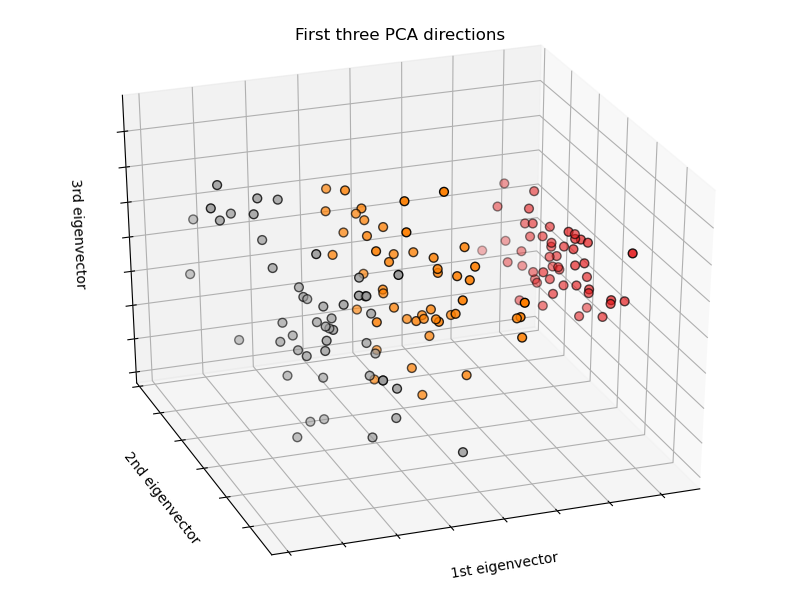
\includegraphics[scale=.4]{iris.png}
        \end{center}
    \end{itemize}
    \end{frame}
    
    \begin{frame}
    \frametitle{Entropy Decision Trees}
        \begin{center}
            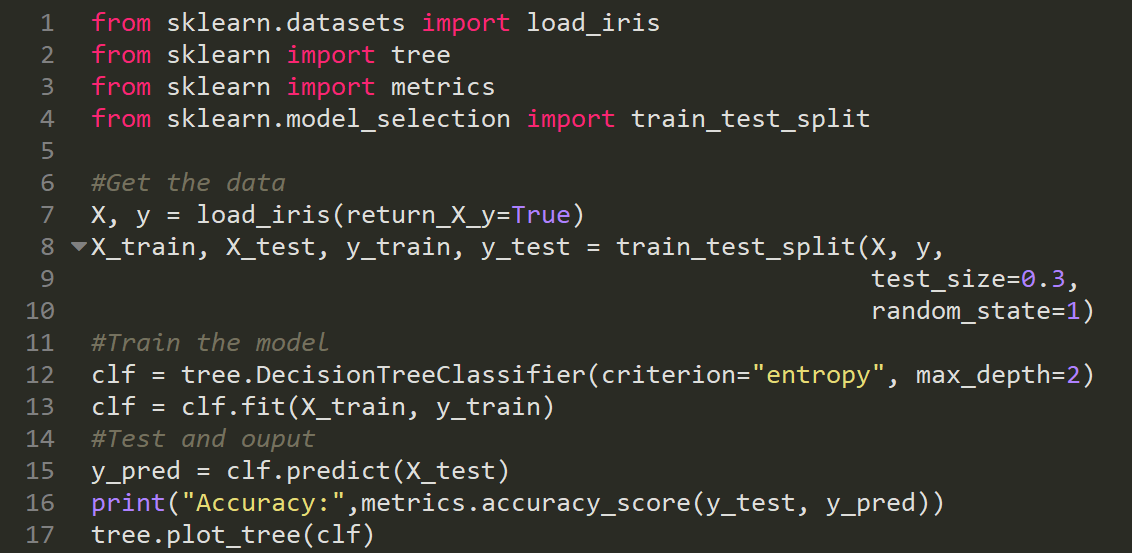
\includegraphics[width=\textwidth]{edtcode.PNG}
        \end{center}
    \end{frame}
    
    \begin{frame}
    \frametitle{Entropy Decision Trees}
        \begin{center}
            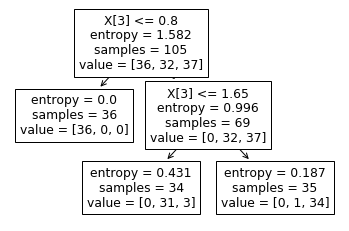
\includegraphics[width=\textwidth]{depth2.png}
        \end{center}
    \end{frame}
    
    \begin{frame}
    \frametitle{Entropy Decision Trees}
        \begin{center}
            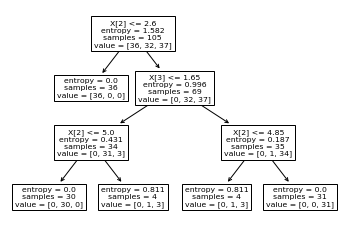
\includegraphics[width=\textwidth]{depth3.png}
        \end{center}
    \end{frame}
    
    \begin{frame}
    \frametitle{Entropy Decision Trees}
        \begin{center}
            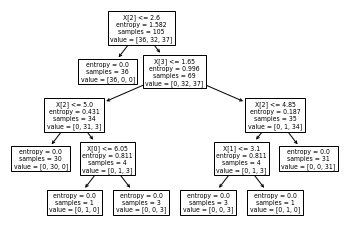
\includegraphics[width=\textwidth]{depth4.png}
        \end{center}
    \end{frame}
    
    \begin{frame}
    \frametitle{Entropy Decision Trees}
        \begin{center}
            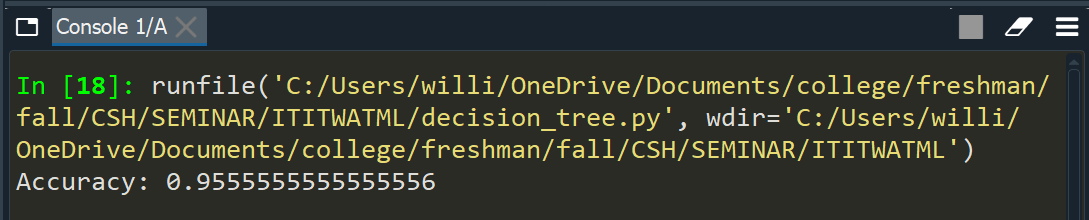
\includegraphics[width=\textwidth]{Ipyth.PNG}
        \end{center}
    \end{frame}
    	
	\subsection{Cross-Entropy as a Cost Function}
	\begin{frame}
	\frametitle{Entropy as a Cost Function}
    	\begin{itemize}
    	    \item Suppose we are attempting binary classification, with a logistic model $$ p(\mathbf{x}) = \frac{1}{1 + \exp \left( \mathbf{w}^\top \mathbf{x}\right)} $$
    	    \pause
    	    \item We have a bunch of observed values, and we want to tune $\mathbf{w}$, but what should we minimize/maximize?
    	    \pause
    	    \item Could try the cross entropy between the model distribution and the observed distribution
    	    \pause  $$ -\sum_{k=1}^N y_k \log(p(x_k)) + (1-y_k)\log(1-p(x_k))$$
    	    \item This is a result called logistic regression. 
    	\end{itemize}
	\end{frame}
	
	\begin{frame}
    \frametitle{Entropy Decision Trees}
        \begin{center}
            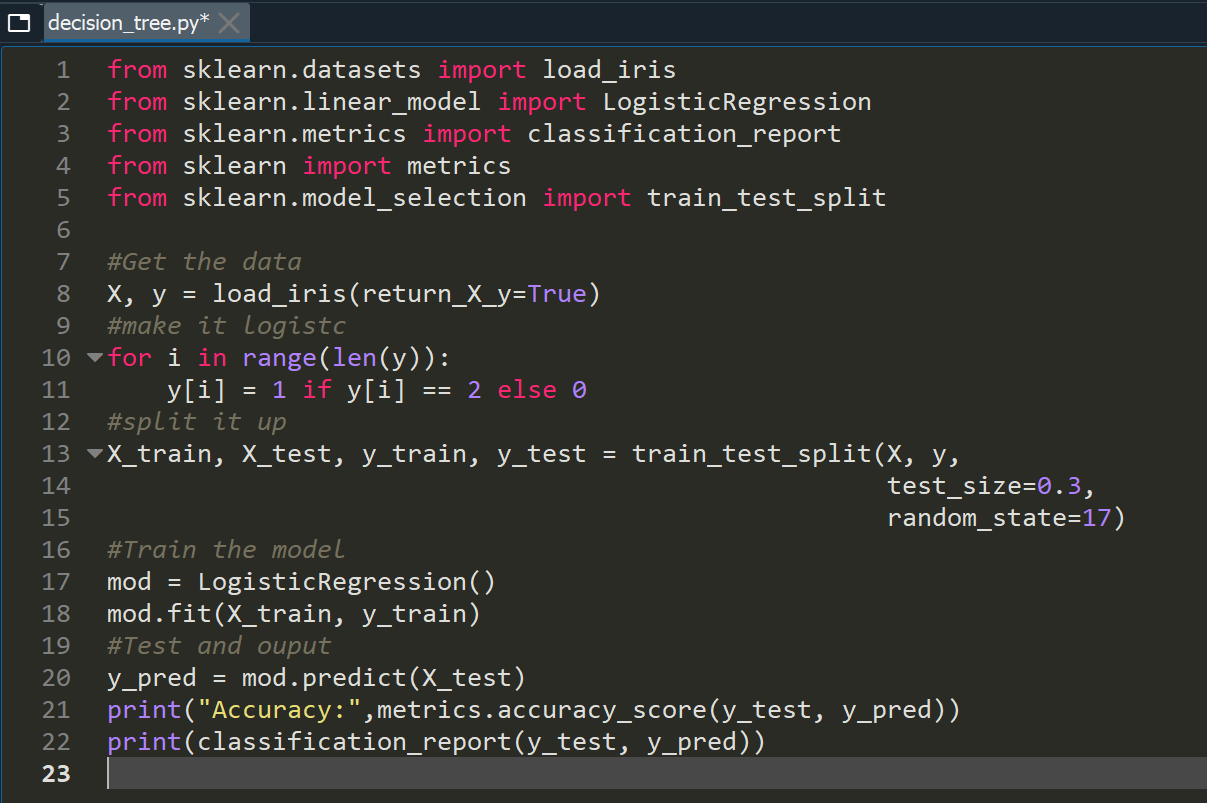
\includegraphics[width=\textwidth]{log_reg.PNG}
        \end{center}
    \end{frame}
    
    \begin{frame}
    \frametitle{Entropy Decision Trees}
        \begin{center}
            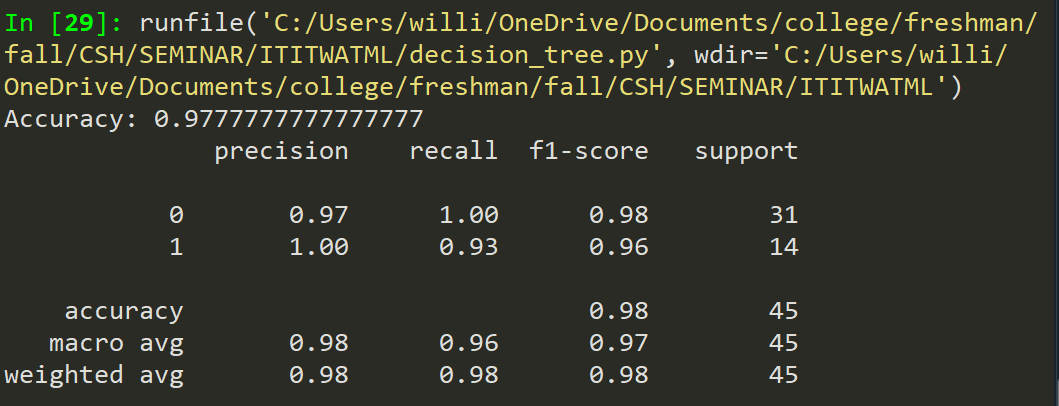
\includegraphics[width=\textwidth]{ipythlr.PNG}
        \end{center}
    \end{frame}
	
	\begin{frame}
	\frametitle{Cross-Entropy as a Cost Function}
	    \begin{itemize}
        	\item This is typically the most important application to machine learning. 
        	\pause
        	\item Neural Networks
        	\pause
        	\item Other models
        	\pause
        	\item Priors for Bayesian Classification
	    \end{itemize}
	\end{frame}
	
	\subsection{Kernel Principle Component Analysis}
	\begin{frame}
	\frametitle{Kernel Principle Component Analysis}
	\begin{itemize}
	    \item Normal PCA, you find the orthogonal projections that maximize the variance of the RV after projection. 
	    \pause 
	    \item Can be computed by Eigendecomposition of the (usually MLE) sample covariance matrix. 
	    \pause 
	    \item In a very complicated sense, if you imagine maximum generalized entropy projections in a special way, one gets out that one could actually does to PCA after mapping to some \textit{feature space}. The inner product in feature space is a measure of closeness, a kernel. 
	    \pause 
	    \item http://citeseerx.ist.psu.edu/ viewdoc/download?doi=10.1.1. 381.288&rep=rep1&type=pdf
	\end{itemize}
	\end{frame}
	
\end{document}